\documentclass[xcolor=svgnames]{beamer}
\hfuzz=200pt
\vfuzz=200pt

\usetheme{Warsaw}
\usecolortheme{dolphin}
\usepackage[T1]{fontenc}
\usepackage{graphicx}
\newtheorem{thm}{Theorem}[section]
\newtheorem{claim}[thm]{Claim}
\newtheorem{conj}[thm]{Conjecture}
\newtheorem{cor}[thm]{Corollary}
\newtheorem{conclusion}{Conclusion}
\newtheorem{qu}[thm]{Question}
\newtheorem{remark}[thm]{Remark}
\newtheorem{prop}[thm]{Proposition}
\newtheorem{prob}[thm]{Problem}
\newtheorem{exam}[thm]{Example}
\newtheorem{defn}[thm]{Definition}
\newcommand{\bra}[1]{\langle #1 |}
\newcommand{\ket}[1]{| #1 \rangle}
\newcommand{\braket}[2]{\langle #1 | #2 \rangle}
\newcommand{\ketbra}[2]{| #1 \rangle\langle #2 |}
\newcommand{\bb}{\mathbb}
\newcommand{\cl}{\mathcal}
\newcommand{\Tr}{{\rm Tr}}
\newcommand{\fA}{\mathfrak{A}}
\renewcommand{\emph}[1]{\textcolor{SeaGreen}{\textbf{#1}}}
\setbeamercovered{transparent}
\setbeamertemplate{navigation symbols}{} % remove navigation symbols

\newcommand{\M}{\mathcal{M}}
\newcommand{\N}{\mathbb{N}}
\newcommand{\Z}{\mathbb{Z}}
\newcommand{\Q}{\mathbb{Q}}
\newcommand{\R}{\mathbb{R}}
\newcommand{\C}{\mathbb{C}}
\newcommand{\F}{\mathbb{F}}

% nice-looking footnotes in slides
\usepackage[absolute,overlay]{textpos} 
\newenvironment{reference}[2]{% 
  \begin{textblock*}{\textwidth}(#1,#2) 
      \footnotesize\it\bgroup\color{red!50!black}}{\egroup\end{textblock*}} 

% matrix norm (triple-bar)
\newcommand{\mnorm}[1]{%
\left\vert\kern-0.9pt\left\vert\kern-0.9pt\left\vert #1
\right\vert\kern-0.9pt\right\vert\kern-0.9pt\right\vert}
\newcommand{\bmnorm}[1]{%
\big\vert\kern-0.9pt\big\vert\kern-0.9pt\big\vert #1
\big\vert\kern-0.9pt\big\vert\kern-0.9pt\big\vert}

\title[\textit{S}-Bandwidth and PST on Quantum Networks]{\textbf{\textit{S}-Bandwidth as an Indicator of Perfect} \\ \textbf{State Transfer on Quantum Networks}}
\author[N.~Johnston, S.~Plosker, \& \emph{L. M. B.~Varona}]{Nathaniel Johnston\inst{\textit{a}}, Sarah Plosker\inst{\textit{b}}, and \emph{Luis M. B. Varona}\inst{\textit{a}} \\[0.25em] 
\includegraphics[width=2.25cm]{misc_graphics/mta_logo.png}\quad\quad\quad\quad
\includegraphics[width=2.25cm]{misc_graphics/brandon_logo.png} \\[-1.25em]}
\institute[AUPAC 2025]{\textit{\inst{a}Mount Allison University\quad\quad\inst{b} Brandon University} \\[4em] Atlantic Undergraduate Physics and Astronomy Conference 2025 \\ Memorial University, St. John's, NL}
\date{February 1, 2025}

\usepackage{amsmath,amsxtra,amssymb,amsthm,amsfonts}
\usepackage{mathtools}
\usepackage{bm}
\usepackage{unicode-math}
\usepackage{tikz}
\setbeamertemplate{caption}[numbered]
\begin{document}

\frame{\titlepage}

%%%%%%%%%%%%%%%%%%%%%%%%%%%%%%%%%%%%%%%%
\section{Background and Preliminaries}
%%%%%%%%%%%%%%%%%%%%%%%%%%%%%%%%%%%%%%%%

	%%%%%%%%%%%%%%%%%%%%%%%%%%%%%%%%%%%%%%%%
	\subsection{Quantum Information Systems}
	%%%%%%%%%%%%%%%%%%%%%%%%%%%%%%%%%%%%%%%%
    
    \frame{
		\frametitle{Quantum Information Systems}
        Whereas classical computers use \emph{bits} ($0$ or $1$), quantum computers use superposed \emph{qubits}. Quantum systems can solve \textit{some} problems far faster\textemdash but they are highly susceptible to decoherence.\medskip
        
        \begin{itemize}
                \uncover<2->{\item A qubit $\ket{\psi} = \alpha\ket{0} + \beta\ket{1}$ is a \emph{superposition} of the classical basis states $\ket{0}$ and $\ket{1}$, where $\lvert\alpha\rvert^2 + \lvert\beta\rvert^2 = 1$ with $\alpha, \beta \in \C$}
            \uncover<3->{\item Recall the famous thought experiment \emph{Schr\"{o}dinger's cat}}:
        \end{itemize}
        
        \begin{figure}
            \centering
            \visible<3->{
\includegraphics[height=3.8cm]{misc_graphics/ash.jpg}}
            \vspace*{-0.3cm}
            \uncover<3->{\caption{My cat, \emph{Ash}. (She may be both \emph{awake} and \emph{asleep}\ldots)}
            \label{fig:fig1}}
        \end{figure}
	}
    
    \frame{
		\frametitle{Quantum Information Systems}
        We use undirected graphs to represent \emph{quantum spin networks} of coupled qubits (typically realized by electrons or photons).\medskip
        
        \begin{itemize}
            \uncover<2->{\item \emph{Vertices} represent qubit particles, \emph{edges} represent couplings, and \emph{edge weights} represent coupling constants/strengths}
            \uncover<3->{\item Movement of information (contained in a particle's quantum state) from one vertex to another is called \emph{state transfer}}
            \uncover<4->{\item A network with quantum couplings between all but two qubits:}
        \end{itemize}
        
        \begin{figure}
            \centering
            \vspace*{-0.05cm}
            \visible<4->{
                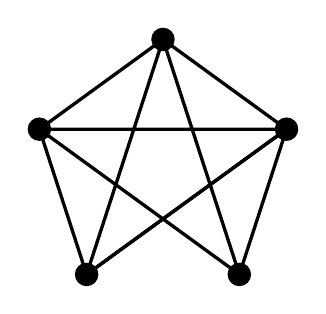
\begin{tikzpicture}
                    \draw[very thick]  (18:1.65) \foreach \a in {90,162,234} { -- (\a:1.65) } -- cycle;
                    \draw[very thick] (18:1.65) \foreach \a in {162,306,90,234} { -- (\a:1.65) } -- cycle;
                    \draw[very thick] (18:1.65) \foreach \a in {306,18} { -- (\a:1.65) };
                    \foreach \a in {18,90,162,234,306} { \node[black,fill=black,circle,inner sep=3pt] at (\a:1.65){}; }
                \end{tikzpicture}
            }
            \vspace*{-0.3cm}
            \uncover<4->{\caption{The complete multipartite graph \emph{$K_{1,1,1,2}$} on 5 vertices.}
            \label{fig:fig2}}
        \end{figure}
	}
    
    %%%%%%%%%%%%%%%%%%%%%%%%%%%%%%%%%%%%%%%%
    \subsection{Perfect State Transfer}
    %%%%%%%%%%%%%%%%%%%%%%%%%%%%%%%%%%%%%%%%
    \frame{
		\frametitle{Perfect State Transfer}
        \begin{defn}[Perfect state transfer]Let $G$ be a quantum network, and let $\Psi_t : V(G) \to \C$ be the wave function of $u \in V(G)$ after a period $t \ge 0$ of unitary evolution (so $\Psi_0(u) = 1$ and $\Psi_0(x) = 0 \ \forall x \ne u$). We say there is \emph{perfect state transfer (PST)} from $u$ to $v \ne u$ if $\exists T > 0$ so that $\lvert\Psi_T(v)\rvert = 1$.\end{defn}
        
        \begin{itemize}
                \uncover<2->{\item \emph{i.e.,} when 100\% of qubit $u$'s initial information state is transferred to qubit $v$ without physical particle motion}
                \uncover<3->{\item To test for PST \textit{specifically} from $u$ to $v$, we can use the \emph{discrete Schr\"{o}dinger's equation} on $G$ for $u$: $\frac{d}{dt}\Psi_t = iH\Psi_t$}
                \uncover<4->{\item But using wave equations to determine whether PST occurs on $G$ between \textit{any} pair of qubits can get very, very messy\ldots}
                \uncover<5->{\item \ldots so we often turn to \emph{matrix mechanics}!}
        \end{itemize}
	}
    
    \frame{
		\frametitle{Perfect State Transfer}
        It is easier to search for PST between arbitrary $x, y \in V(G)$ with \emph{unitary operators} rather than set up $\lvert V(G) \rvert$ wave equations.\medskip
        
        \begin{itemize}
                \uncover<2->{\item \emph{e.g.,} the \emph{transition matrix} $U_t = e^{itA(G)}$ models \emph{unitary evolution} on $G$ in the total absence of noise (where $A(G)$ is the adjacency matrix of $G$)}
                \uncover<3->{\item There is PST on $G$ iff $\exists T > 0$ and $x, y \in V(G)$ so that $\lvert\bra{x}U_T\ket{y}\rvert = 1$, where $\ket{x}, \ket{y}$ are the \emph{initial states} of $x, y$}
                \uncover<4->{\item Now we only need the fixed initial states $\{\ket{x} : x \in V(G)\}$ instead of a new time-variant wave function for each particle}
                \uncover<5->{\item Perfectly unitary evolution (and hence PST) is impossible in practice due to quantum noise, but we \textit{can} achieve \emph{pretty good state transfer (PGST)} (as high as $>\!97\%$ fidelity!)}
        \end{itemize}
	}
    
    \frame{
		\frametitle{Perfect State Transfer}
        The (unweighted) cycle graph on $4$ vertices represents a quantum network with PST from node $1$ to node $3$. (We will see later that it is also something called \emph{Hadamard diagonalizable}.)\medskip
        
        \begin{figure}
            \begin{minipage}[b]{.45\textwidth}
                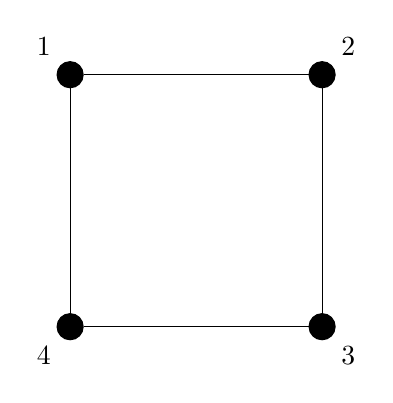
\begin{tikzpicture}
                    \node[circle, draw, fill=black] (1) [label=north west:1] at (0, 3.2) {};
                    \node[circle, draw, fill=black] (2) [label=north east:2] at (3.2, 3.2) {};
                    \node[circle, draw, fill=black] (3) [label=south east:3] at (3.2, 0) {};
                    \node[circle, draw, fill=black] (4) [label=south west:4] at (0, 0) {};
                    \draw (1) -- (2) -- (3) -- (4) -- (1);
                \end{tikzpicture}
                \vspace*{-0.2cm}
                \caption{The cycle graph \emph{$C_4$} exhibits perfect state transfer.}
                \label{fig:fig3}
            \end{minipage}\hfill
            \begin{minipage}[b]{.45\textwidth}
                \centering
                \begingroup
                    \setlength\arraycolsep{6pt}
                    \Large{\(\begin{pmatrix*}[l]
                        \phantom{-}2 & -1 & \phantom{-}0 & -1 \\[3pt]
                        -1 & \phantom{-}2 & -1 & \phantom{-}0 \\[3pt]
                        \phantom{-}0 & -1 & \phantom{-}2 & -1 \\[3pt]
                        -1 & \phantom{-}0 & -1 & \phantom{-}2
                    \end{pmatrix*}\)}
                \endgroup
                \vspace*{0.6cm}
                \caption{The \emph{Laplacian matrix} $L(C_4) \coloneqq D(C_4) - A(C_4)$.}
                \label{fig:fig4}
            \end{minipage}
        \end{figure}
	}
    
    \frame{
		\frametitle{Perfect State Transfer}
        \begin{figure}
            \centering
            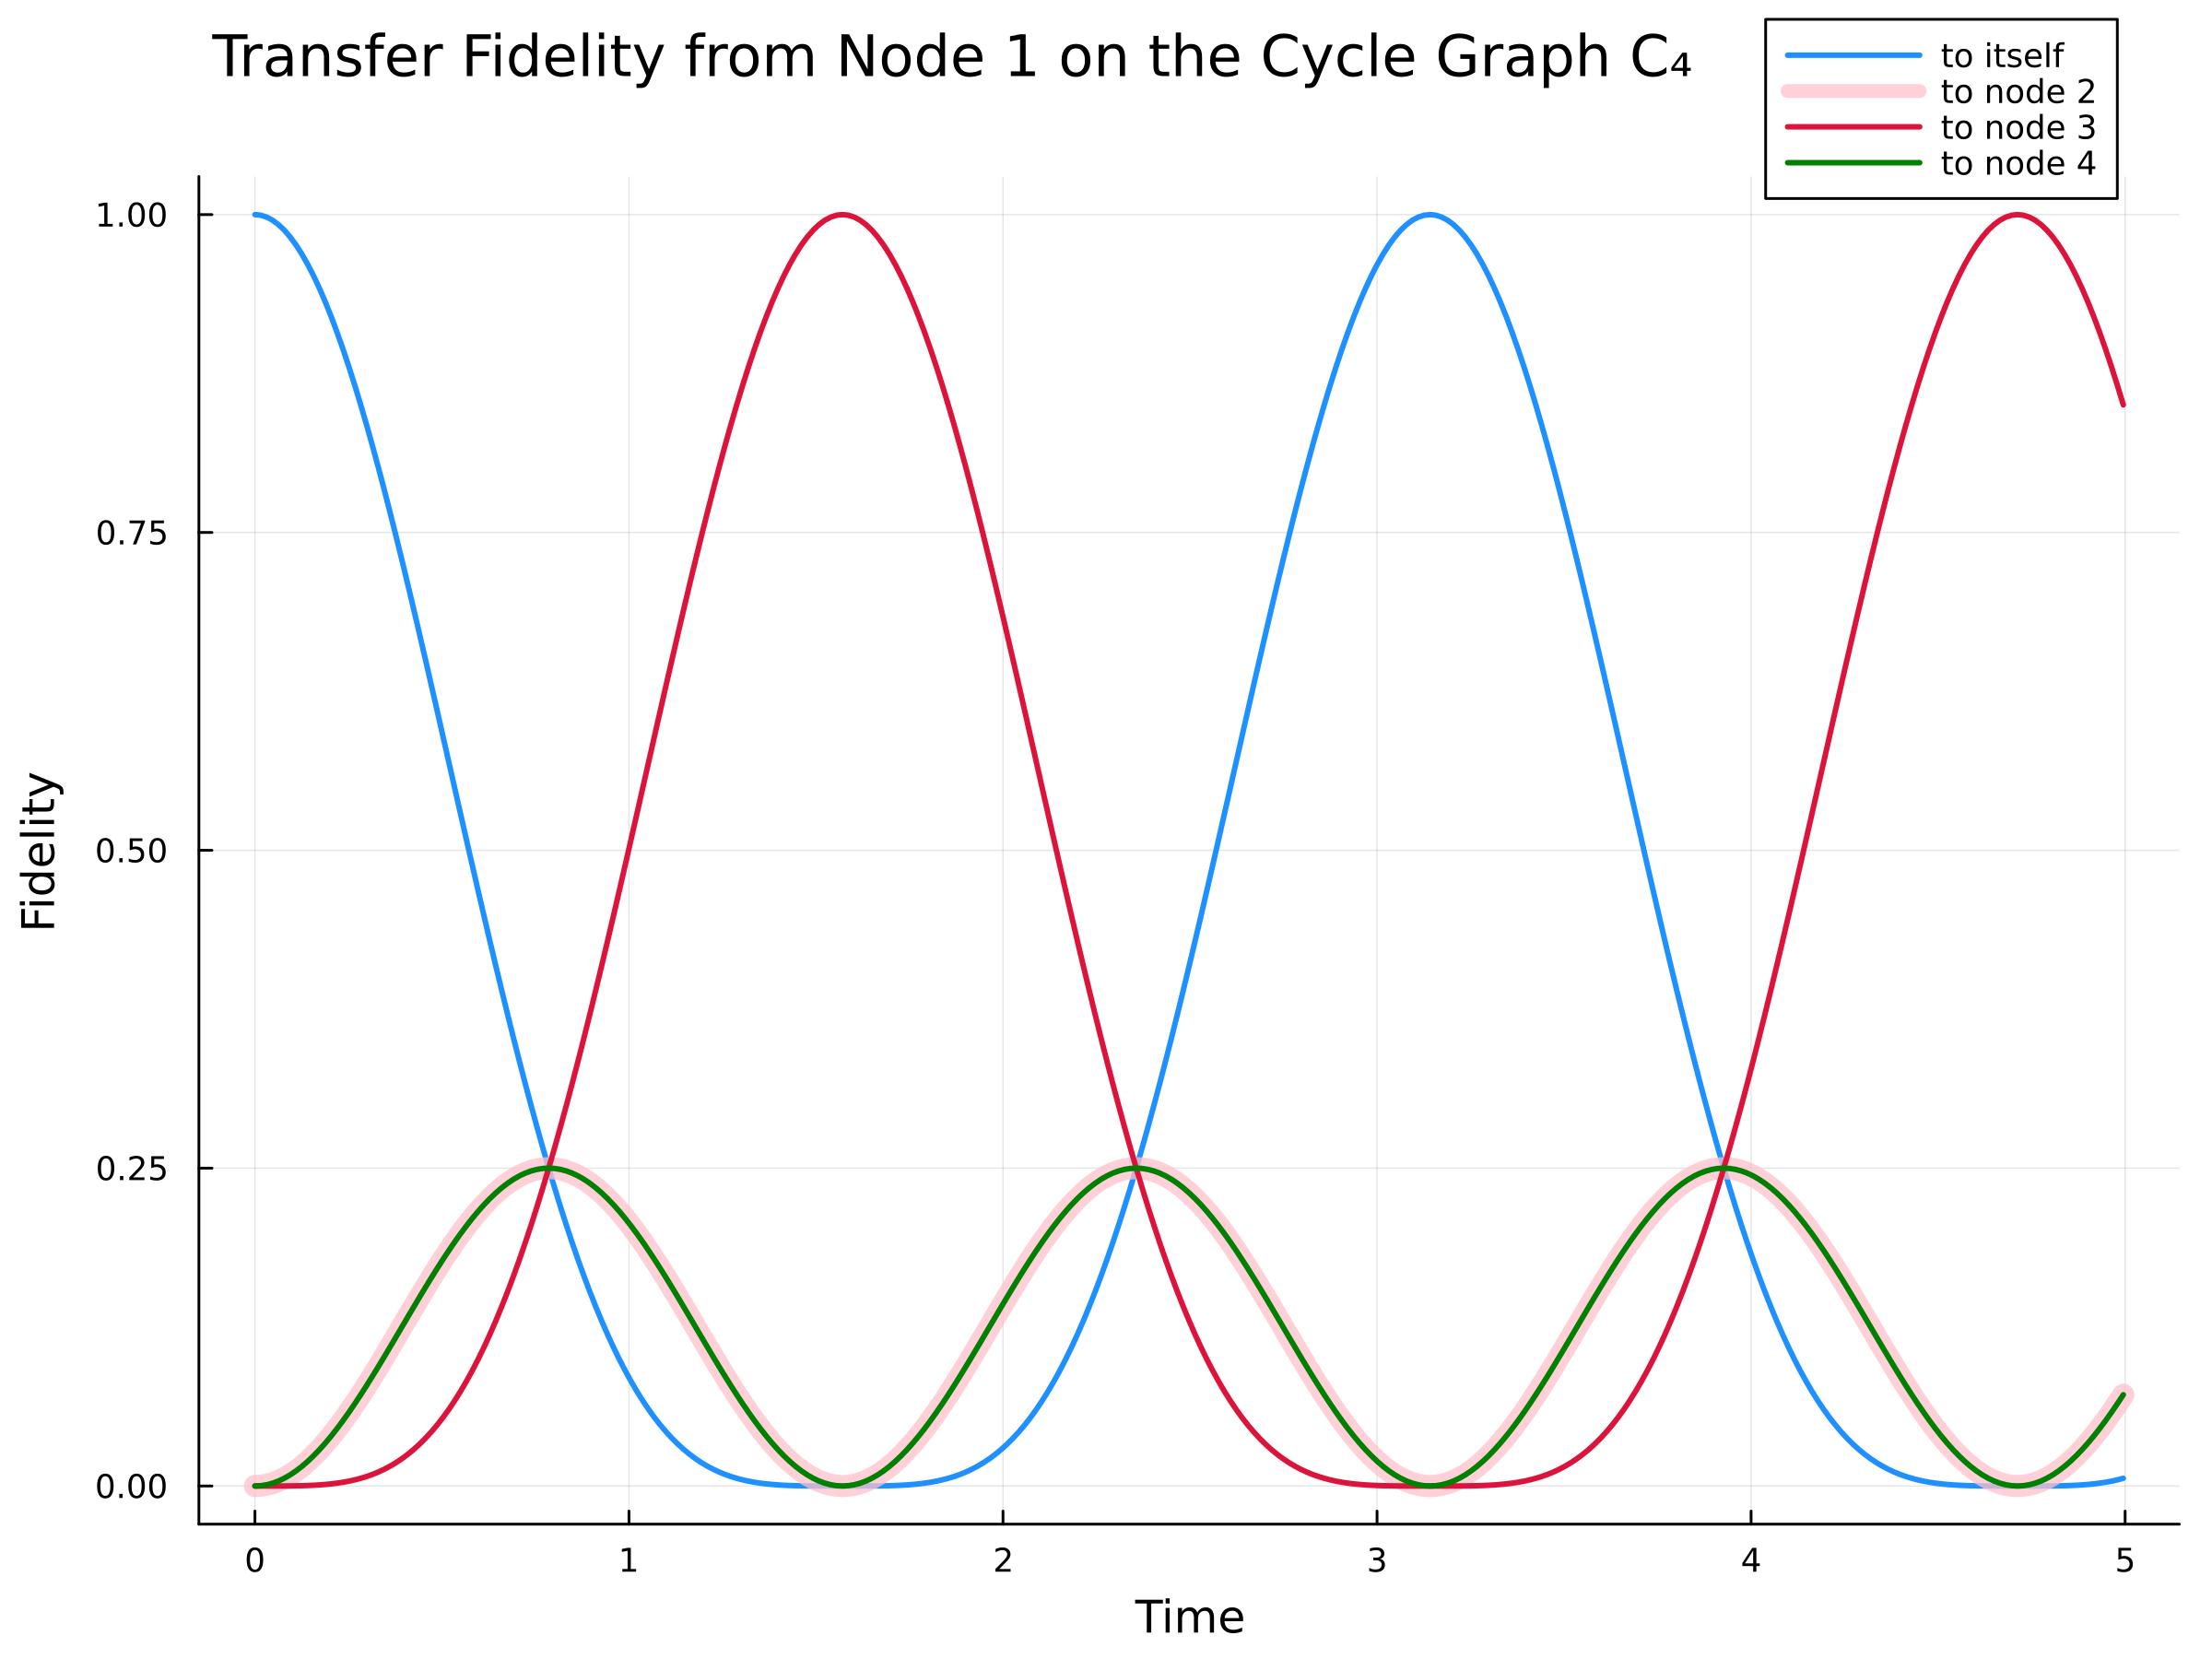
\includegraphics[height=7cm]{pst_code_plots/c4_transfer_fidelity.png}
            \vspace*{-0.4cm}
            \caption{A visualization of PST on $C_4$ from node $1$ to node $3$.}
            \label{fig:fig5}
        \end{figure}
	}
    
    \frame{
		\frametitle{Perfect State Transfer}
        \begin{figure}
            \centering
            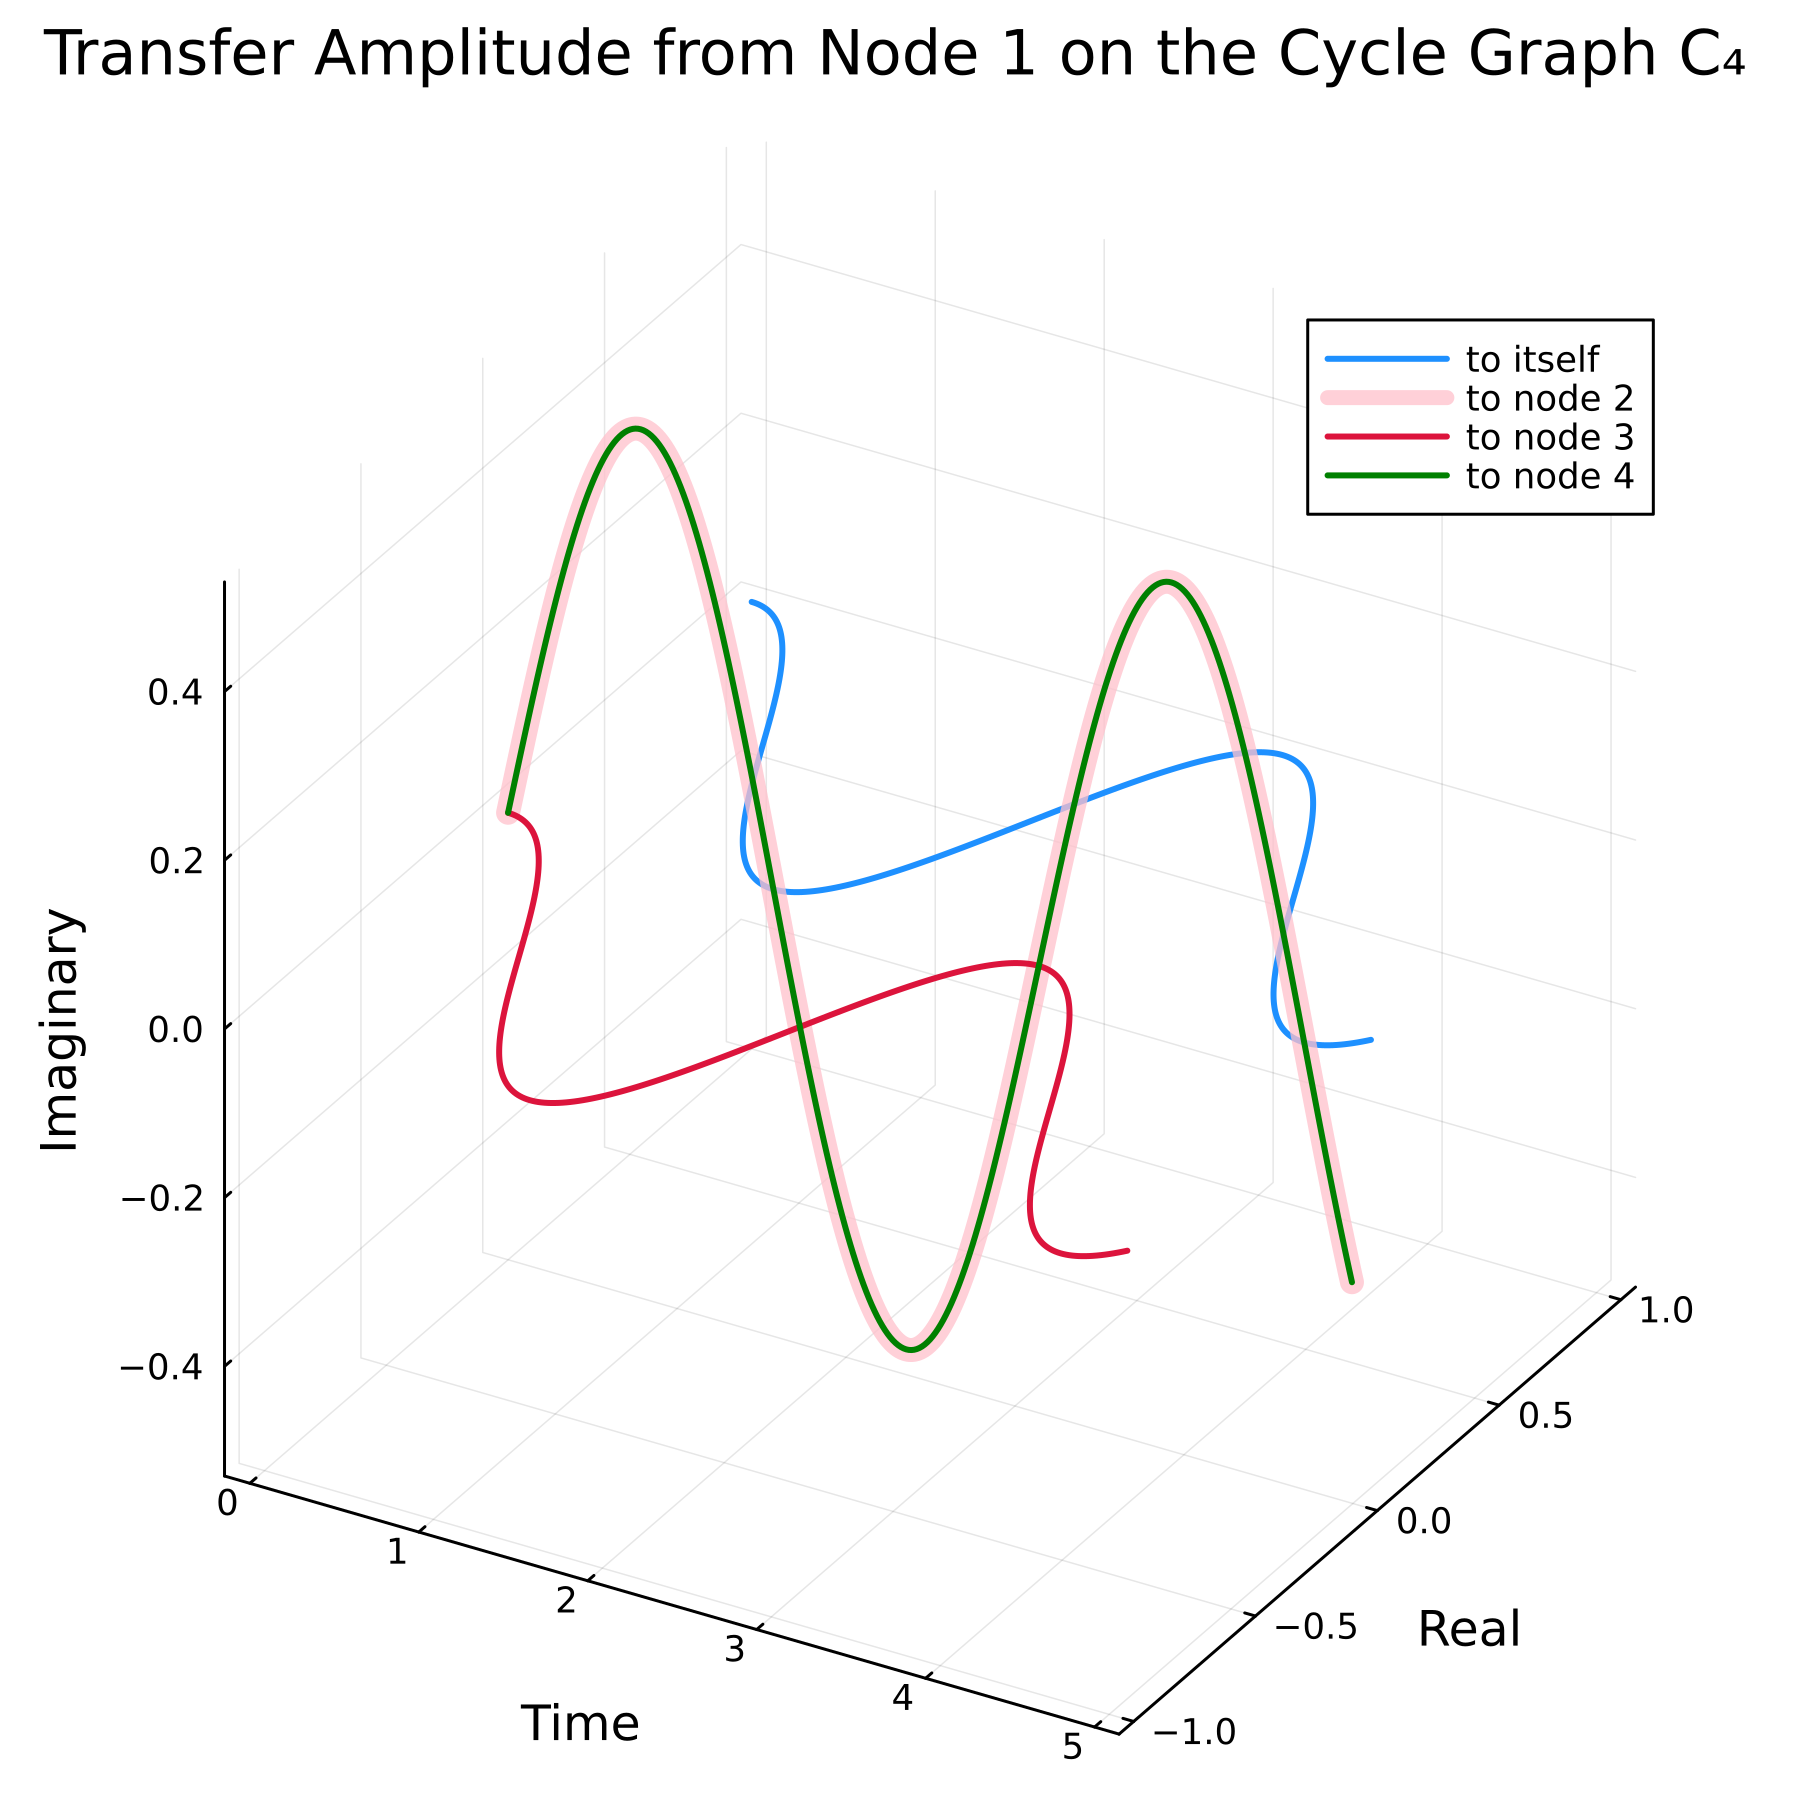
\includegraphics[height=7cm]{pst_code_plots/c4_transfer_amplitude.png}
            \vspace*{-0.4cm}
            \caption{Probability amplitudes of node $1$'s wave function are \emph{complex}\ldots}
            \label{fig:fig6}
        \end{figure}
	}

%%%%%%%%%%%%%%%%%%%%%%%%%%%%%%%%%%%%%%%%
\section{\textit{S}-Bandwidths and State Transfer}
%%%%%%%%%%%%%%%%%%%%%%%%%%%%%%%%%%%%%%%%

	%%%%%%%%%%%%%%%%%%%%%%%%%%%%%%%%%%%%%%%%
	\subsection{\textit{S}-Diagonalizability/\textit{S}-Bandwidth}
	%%%%%%%%%%%%%%%%%%%%%%%%%%%%%%%%%%%%%%%%
    
    \frame{
        \frametitle{$S$-Diagonalizability/$S$-Bandwidth}
        Many of the graphs confirmed to exhibit PST also happen to be \emph{$\{-1,1\}$-} and \emph{$\{-1,0,1\}$-diagonalizable} (for reasons yet unknown):
        
        \uncover<2->{\begin{defn}[$S$-diagonalizability]A graph $G$ on $n$ vertices is called \emph{$S$-diagonalizable} if its Laplacian $L(G)$ is diagonalizable by some matrix with entries from $S \subset \Z$\textemdash{} i.e., if $\exists P \in S^{n \times n}$ and diagonal $D \in \R^{n \times n}$ with $L(G) = PDP^{-1}$.\end{defn}}
        \uncover<3->{In particular, PST graphs tend to have low ($\le\!2$) \emph{$S$-bandwidths}:}    
        \uncover<4->{\begin{defn}[$S$-bandwidth]Define $\beta : \mathcal{M} \to \N$ by $\beta(X) \coloneqq \min\{k : \lvert i - j \rvert \ge k \implies x_{ij} = 0\}$ (some texts use $\lvert i - j \rvert > k$ instead). The \emph{$S$-bandwidth} of a graph $G$ on $n$ vertices, denoted by $\beta_S(G)$, is then the minimum integer $k$ so that $\exists P \in S^{n \times n}$ with $\beta(P^TP) = k$ and $L(G) = PDP^{-1}$.
        \end{defn}\medskip}
    }
    
    \frame{
        \frametitle{$S$-Diagonalizability/$S$-Bandwidth}
        That is, $\beta_S(G) = k$ if and only if $k$ is the smallest integer for which the Laplacian matrix $L(G) \coloneqq D(G) - A(G)$ has a full collection of eigenvectors $\mathbf{v}_1, \ldots, \mathbf{v}_n \in S^{n}$ with $\vert i - j \vert \ge k \implies \langle\mathbf{v}_i, \mathbf{v}_j\rangle = 0$.\medskip
        
        \begin{itemize}
            \uncover<2->{\item Of particular interest are \emph{Hadamard} and \emph{weak Hadamard diagonalizability} ($\beta_{\{-1,1\}}(G) = 1$ and $\beta_{\{-1,0,1\}}(G) \le 2$)}
            \uncover<3->{\item We are investigating \textit{why} qubit couplings in HD/WHD graphs (such as \emph{$C_4$}) are more conducive to high-fidelity transfer}
            \uncover<4->{\item For now, we treat HD/WHD as a heuristic indicator of PST\ldots{} motivating our \emph{novel algorithm} to compute $S$-bandwidth (feasible for any graph on $n \le 18$ vertices!)}
        \end{itemize}
    }
    
	%%%%%%%%%%%%%%%%%%%%%%%%%%%%%%%%%%%%%%%%
	\subsection{Algorithm for \textit{S}-Bandwidth}
	%%%%%%%%%%%%%%%%%%%%%%%%%%%%%%%%%%%%%%%%
    
    \frame{
        \frametitle{Algorithm for $S$-Bandwidth}
        Given some undirected (and possibly weighted) graph $G$ with Laplacian matrix $L \in \R^{n \times n}$, here is an overview of our algorithm:
        
        \begin{itemize}
            \uncover<2->{\item \emph{First:} Validate that the unique eigenvalues $\lambda_1, \lambda_2, \ldots, \lambda_k$ of $L$ are all integers. Iterate over all $\{-1,0,1\}$-vectors $\mathbf{v} \in \R^n$ (unique up to span) and \emph{test $L\mathbf{v} = \lambda_i\mathbf{v}$} for $i \in \{1, 2, \ldots, k\}$.}
            \uncover<3->{\item \emph{Next:} With $V_i$ denoting the matrix whose columns are all the $\{-1,0,1\}$-eigenvectors for $\lambda_i$, \emph{use RREF on each $V_i$} to see if each eigenspace has a linearly independent $\{-1,0,1\}$-basis.}
            \uncover<4->{\item \emph{Third:} If $G$ \textit{is} diagonalizable, construct a basis with minimum Gramian bandwidth for each eigenspace by \emph{recursively adding/eliminating vectors}. Identify \emph{$\beta_{\{-1,0,1\}}(G)$}.}
            \uncover<5->{\item \emph{Last:} By tracking which $\{-1,0,1\}$-eigenvectors are also $\{-1,1\}$-vectors, we can simultaneously determine \emph{$\beta_{\{-1,1\}}(G)$}.}
        \end{itemize}
    }

%%%%%%%%%%%%%%%%%%%%%%%%%%%%%%%%%%%%%%%%
\section{Numerical Results and Future Work}
%%%%%%%%%%%%%%%%%%%%%%%%%%%%%%%%%%%%%%%%

	%%%%%%%%%%%%%%%%%%%%%%%%%%%%%%%%%%%%%%%%
	\subsection{Available \textit{S}-Bandwidth Data}
	%%%%%%%%%%%%%%%%%%%%%%%%%%%%%%%%%%%%%%%%
    
    \frame{
        \frametitle{Available $S$-Bandwidth Data}
        We have tabulated the $\{-1,1\}$- and $\{-1,0,1\}$-bandwidths of:\medskip
        
        \begin{itemize}
            \uncover<2->{\item All unweighted, connected $\{-1,0,1\}$-diagonalizable graphs on $n \leq 11$ vertices}
            \uncover<3->{\item All unweighted, connected, regular/bipartite $\{-1,0,1\}$-diagonalizable graphs on $n \leq 14$ vertices}
            \uncover<4->{\item All (non-uniformly) positively weighted, connected WHD graphs on $n \leq 5$ vertices \textendash\ surprisingly, there are none!\medskip}
        \end{itemize}
        
        \uncover<5->{With regards to pure graph theory \textendash\ we are working on several theorems regarding \emph{bipartiteness} and \emph{graph compositions}.\medskip}
        \uncover<6->{With regards to numerics \textendash\ we are using linear programming to investigate \emph{WHD-inducing edge weights} for higher-order graphs.\medskip}
    }
    
    \frame{
        \frametitle{Available $S$-Bandwidth Data}
        \begin{figure}
            \centering
            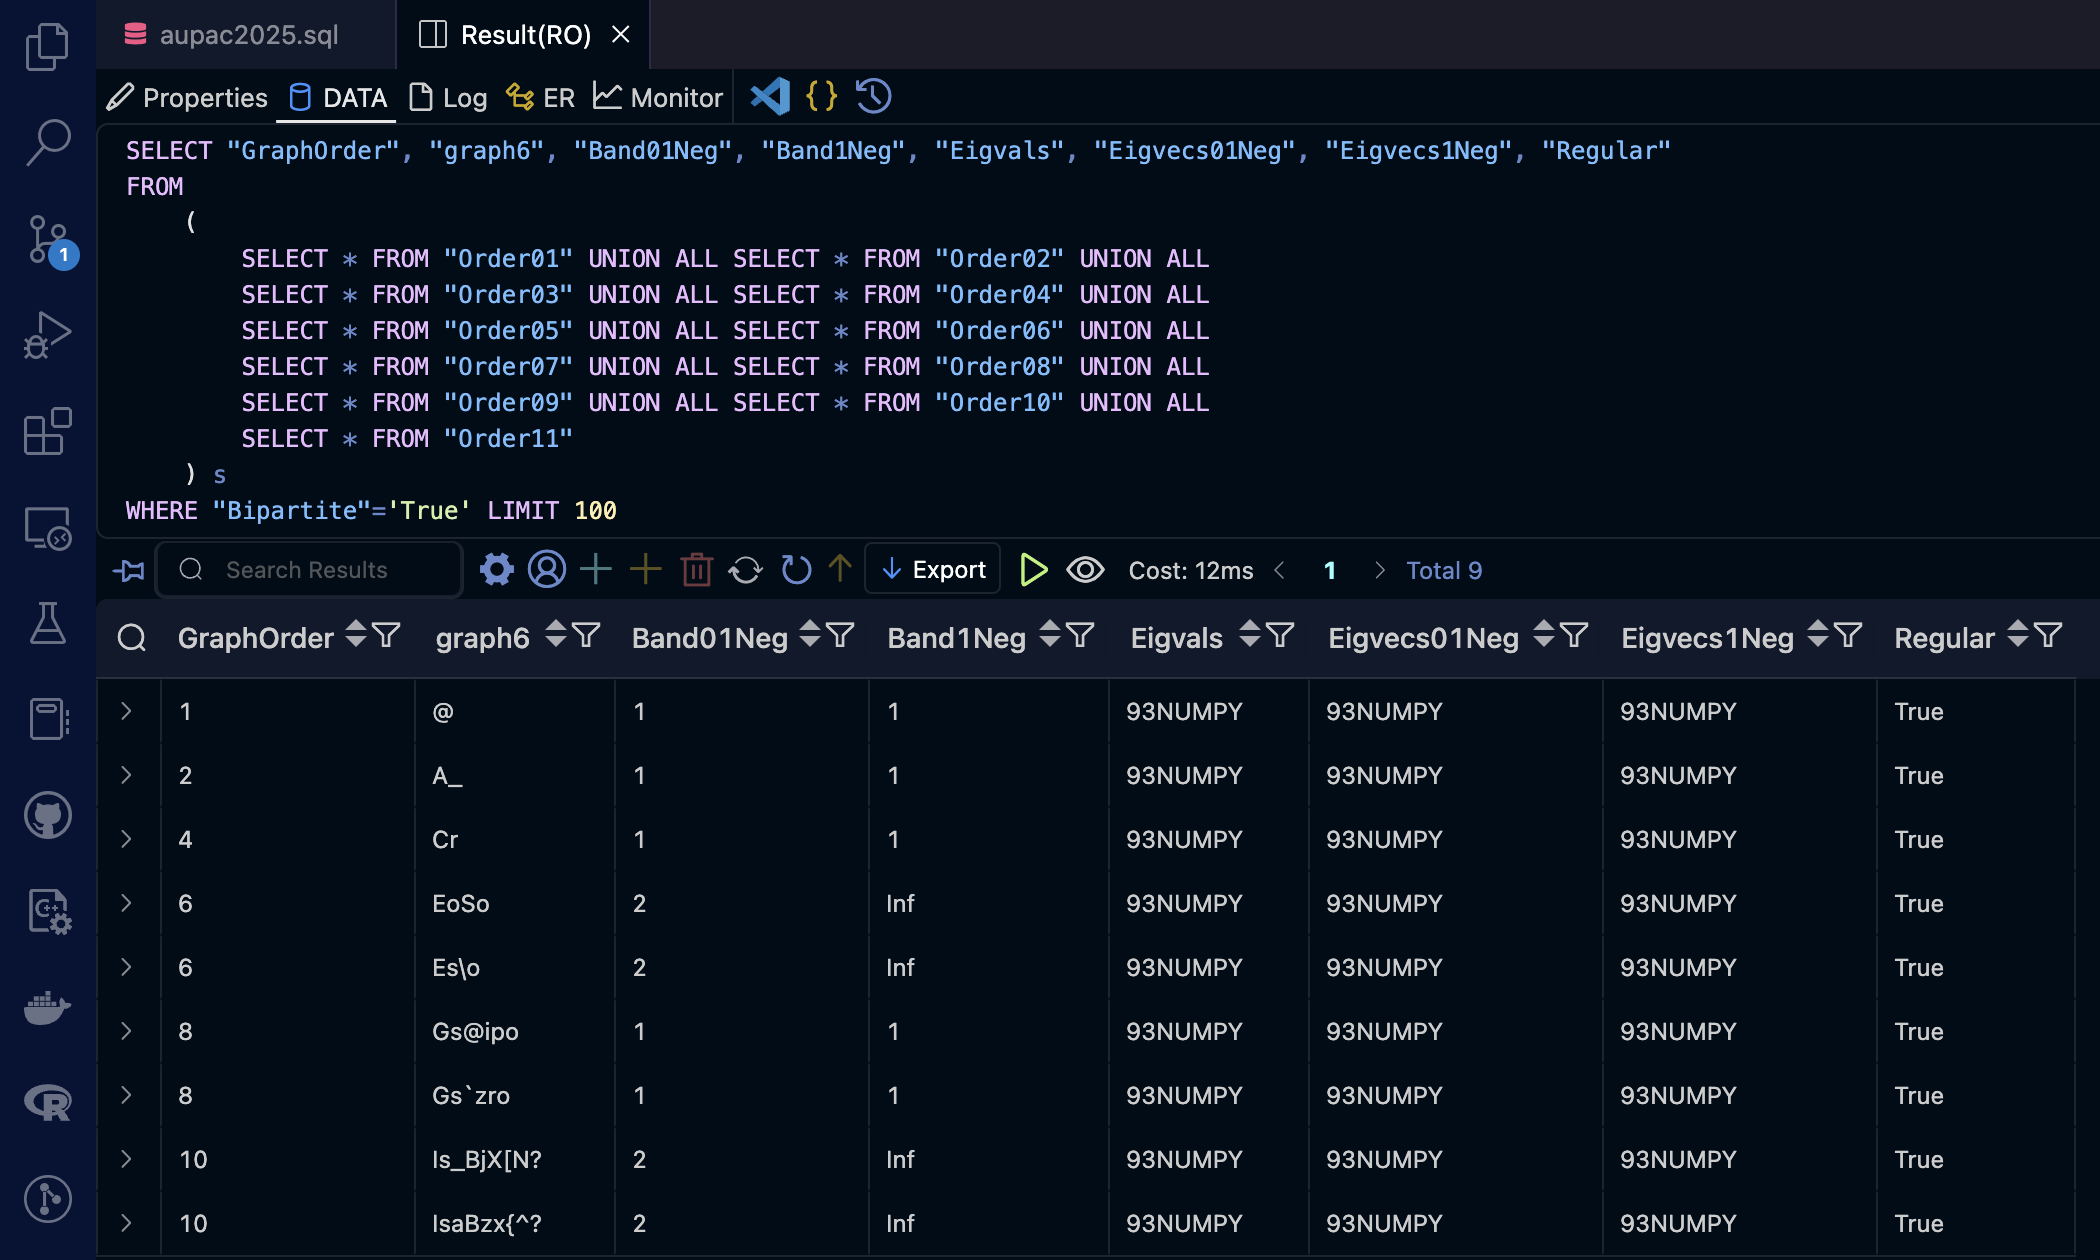
\includegraphics[height=6.3cm]{graph_data_sc/graph_data.png}
            \vspace*{-0.2cm}
            \caption{\textit{Conjecture.} If an (unweighted and connected) \emph{bipartite graph} $G$ is $\{-1,0,1\}$-diagonalizable, then \emph{$G$ is regular} and \emph{$\lvert G \rvert$ is even or $1$.}}
            \label{fig:fig7}
        \end{figure}
    }
    
	%%%%%%%%%%%%%%%%%%%%%%%%%%%%%%%%%%%%%%%%
	\subsection{Thank you!}
	%%%%%%%%%%%%%%%%%%%%%%%%%%%%%%%%%%%%%%%%
    
    \frame{
        \frametitle{Thank you!}
            \begin{figure}
                \centering
                
\includegraphics[height=6.9cm]{misc_graphics/pusheen_thank_you.png}
                \vspace*{-0.3cm}
                \caption{Pusheen the Cat \textless 3}
                \label{fig:fig8}
            \end{figure}
    }

\end{document}